Este capítulo apresenta a revisão sistemática de literatura que fundamenta a pesquisa. O objetivo é situar o problema de disparidade racial em reconhecimento facial no interior de suas linhas de investigação históricas, identificar os limites empíricos e teóricos atualmente atingidos por cada linha e, a partir dessa síntese, mapear explicitamente as lacunas científicas que motivam a proposta metodológica formalizada nos capítulos subsequentes.

A revisão resultou em um corpus de \textbf{104 fichas bibliográficas}, cuja distribuição temporal se concentra na fronteira do conhecimento: aproximadamente 53\,\% das fichas correspondem a publicações de 2024 ou posteriores. Entre as contribuições mais recentes destacam-se cinco pré-\emph{prints} de 2026 --- \emph{SkinToneNet}~\cite{matias2026large}, \emph{IndicFairFace}~\cite{mohsin2026indicfairfac} e trabalhos correlatos~\cite{lian2026closed,ozturk2026demographic,tan2026benchmarking} ---, os artigos de conferência ACM FAccT~2025 e CVPR~2024 (respectivamente \emph{Bayesian Network-informed Meta Reweighting} de \citeonline{liu2025component} e FairCLIP de \citeonline{luo2024fairclip}) e o \emph{FaceScanPaliGemma}~\cite{aldahoul2024exploring}, disponibilizado como pré-print arXiv em outubro de 2024 e posteriormente publicado no \emph{Nature Scientific Reports}. Esse núcleo contemporâneo é complementado por marcos canônicos de fundamentação teórica --- \citeonline{buolamwini2018gender}, \citeonline{perez2018film}, \citeonline{hardt2016equality} e \citeonline{kleinberg2017inherent} --- e por três aportes disciplinares externos à ciência da computação: antropologia biológica~\cite{lewontin1972apportionmen,fuentes2019aapa}, sociologia latino-americana~\cite{telles2014pigmentocrac} e sociologia identitária~\cite{lopez2017hispanic}.

A organização do capítulo segue seis frentes teórico-empíricas, uma revisão dos paradigmas arquiteturais de \emph{backbone}, uma fundamentação formal de métricas, uma frente instrumental e o mapeamento final de lacunas. As Seções~\ref{sec:rl_datasets} a~\ref{sec:rl_fairrep} percorrem, em ordem cronológica de emergência na literatura, as respostas historicamente propostas ao problema de \emph{fairness} --- termo aqui definido como paridade de desempenho entre grupos demográficos, na acepção formal de \citeonline{hardt2016equality} adotada ao longo do trabalho. A Seção~\ref{sec:rl_backbones} apresenta os dois paradigmas arquiteturais contemporâneos para classificação facial --- o convolucional (linha ResNet e sua modernização ConvNeXt) e o baseado em atenção (Vision Transformers) ---, contextualizando a escolha do ConvNeXt-T adotada nesta pesquisa. A Seção~\ref{sec:rl_metricas} apresenta as métricas formais de \emph{fairness} \emph{group-level} e o Teorema da Impossibilidade de \citeonline{kleinberg2017inherent}, que motivam o princípio metodológico de triangulação de métricas adotado no Capítulo~\ref{chapter:metodologia}. A Seção~\ref{sec:rl_arquit} apresenta a frente instrumental de auditoria automatizada de datasets e de mecanismos arquiteturais de \emph{conditioning}. A Seção~\ref{sec:rl_conditioning_alt} discute alternativas de \emph{conditioning} ponderadas antes da escolha metodológica final. A Seção~\ref{sec:rl_gaps} sintetiza as cinco lacunas científicas identificadas no corpus, as quais orientam diretamente os objetivos formulados no Capítulo~\ref{chapter:objetivos}.

\section{Balanceamento de dados}
\label{sec:rl_datasets}

A primeira geração de respostas ao problema de \emph{fairness} facial consistiu em \textbf{datasets balanceados por design}, ou seja, conjuntos de imagens construídos com a preocupação explícita de manter proporções semelhantes de amostras entre categorias demográficas sensíveis --- especialmente raça e gênero. A premissa subjacente, herdada da estatística clássica, é a de que representações equilibradas no treinamento produziriam desempenho igualmente equilibrado no teste.

O primeiro marco dessa geração foi o \emph{Racial Faces in-the-Wild} (RFW)~\cite{wang2019racial}, que balanceia quatro categorias no protocolo de \emph{verificação um-para-um}, isto é, na decisão binária de se duas imagens correspondem à mesma identidade. Em seguida, o \emph{Balanced Faces in the Wild} (BFW)~\cite{robinson2020face} cobriu oito subgrupos formados pelo cruzamento de raça e gênero. O FairFace~\cite{karkkainen2021fairface}, no ano seguinte, ampliou a granularidade racial para sete categorias (\emph{White}, \emph{Black}, \emph{Indian}, \emph{East Asian}, \emph{Southeast Asian}, \emph{Middle Eastern} e \emph{Latinx/Hispanic}) em 108.501 imagens, tornando-se o \emph{benchmark} de referência para classificação racial multi-classe adotada nesta pesquisa. Também em 2021 foi lançado o \emph{Casual Conversations}~\cite{hazirbas2021towards}, expandido posteriormente na versão v2~\cite{porgali2023casual}, que agregou anotações de \emph{self-reported gender} (identidade de gênero declarada pelo próprio participante) e idade, juntamente com rotulagem de tom de pele nas escalas Fitzpatrick e Monk Skin Tone realizada por anotadores previamente treinados, cobrindo sete países.

Apesar da consolidação dessa geração de datasets, a persistência da disparidade específica de \emph{Latinx} no FairFace, discutida no Capítulo~\ref{chapter:introducao}, evidenciou que o balanceamento amostral, embora condição necessária, não é condição suficiente para mitigar o gap. O reconhecimento explícito dessa insuficiência --- corroborado pelos estudos empíricos de \citeonline{kolla2022impact} e pelas observações metodológicas de \citeonline{wang2019racial} --- deslocou o foco da comunidade científica das intervenções sobre os dados para as intervenções sobre o algoritmo, discutidas na seção seguinte.


\section{Mitigação algorítmica}
\label{sec:rl_mitigacao}

Diante da insuficiência do balanceamento amostral, a comunidade científica consolidou uma segunda geração de respostas ao problema, deslocando o esforço para o \textbf{processo de otimização dos modelos}. As técnicas dessa geração agem em três frentes complementares: a \emph{loss functions}, a arquitetura do classificador e o próprio \emph{fine-tuning}, isto é, o ajuste dos pesos de um modelo pré-treinado sobre a tarefa-alvo. Apresentam-se a seguir, os trabalhos que estruturam essa geração e que servirão como \emph{baselines} de comparação para a proposta metodológica desta pesquisa.

A linha inaugural é a do \emph{adversarial debiasing}, estabelecida por \citeonline{zhang2018mitigating}: um segundo modelo (o adversário) é treinado para prever o atributo sensível a partir das \emph{features} internas do classificador principal, forçando este último a produzir representações das quais o atributo demográfico não seja mais recuperável. Trata-se de referência ainda hoje amplamente utilizada como \emph{baseline} de mitigação. Dois anos depois, \citeonline{sagawa2020distribution} formalizaram a \emph{Distributionally Robust Optimization} (DRO) sobre grupos, técnica que substitui a minimização do erro médio pela minimização do erro do \emph{grupo demográfico de pior desempenho} (\emph{worst-case group}), oferecendo garantia formal de desempenho para o subgrupo mais penalizado.

\citeonline{park2022fair} propuseram o \emph{Fair Supervised Contrastive Learning} (FSCL+), extensão do \emph{Supervised Contrastive Learning} (SupCon) --- técnica que agrupa, no espaço de representação, amostras da mesma classe e afasta amostras de classes diferentes ---, demonstrando formalmente que o SupCon padrão, quando aplicado sobre datasets enviesados, incentiva os \emph{encoders} (as camadas responsáveis por transformar imagens em vetores de \emph{features}) a codificarem indiretamente atributos demográficos, propagando o viés para as camadas posteriores. No mesmo ano, \citeonline{lin2022fairgrape} introduziram o FairGRAPE, técnica de \emph{pruning fairness-aware} que remove seletivamente conexões redundantes da rede neural com controle explícito do impacto sobre subgrupos demográficos; nesse mesmo trabalho, os autores documentaram independentemente o \emph{baseline} canônico de 72\,\% de acurácia agregada da arquitetura ResNet-34 sobre a classificação racial de sete classes do FairFace em regime \emph{in-domain}, isto é, com treino e teste sobre partições do mesmo dataset.

As contribuições mais recentes deslocaram a discussão para arquiteturas Pareto-eficientes e para métricas alternativas de equidade. \citeonline{manzoor2024fineface} propuseram o FineFACE, arquitetura baseada em \emph{cross-layer mutual attention learning} --- mecanismo que permite às camadas de diferentes profundidades trocarem informação por meio de atenção mútua ---, atingindo operação \emph{Pareto-eficiente} no dataset CelebA, isto é, configurações em que não se pode melhorar acurácia sem piorar \emph{fairness}, e vice-versa. Em 2025, \citeonline{liu2025component}, em publicação na conferência ACM FAccT, propuseram o \emph{Bayesian Network-informed Meta Reweighting}, introduzindo a noção de \emph{face component fairness} --- equidade avaliada componente a componente do rosto (olhos, nariz, boca) --- como \emph{surrogate}, ou seja, aproximação operacional mais mensurável, para a noção abstrata de \emph{demographic fairness}.

A Figura~\ref{fig:timeline-mitigacoes} sintetiza cronologicamente as seis contribuições, agrupando-as por categoria metodológica.

\begin{figure}[htbp]
\centering
\caption{Linha do tempo das principais contribuições em mitigação algorítmica de viés (2018--2025).}
\centering
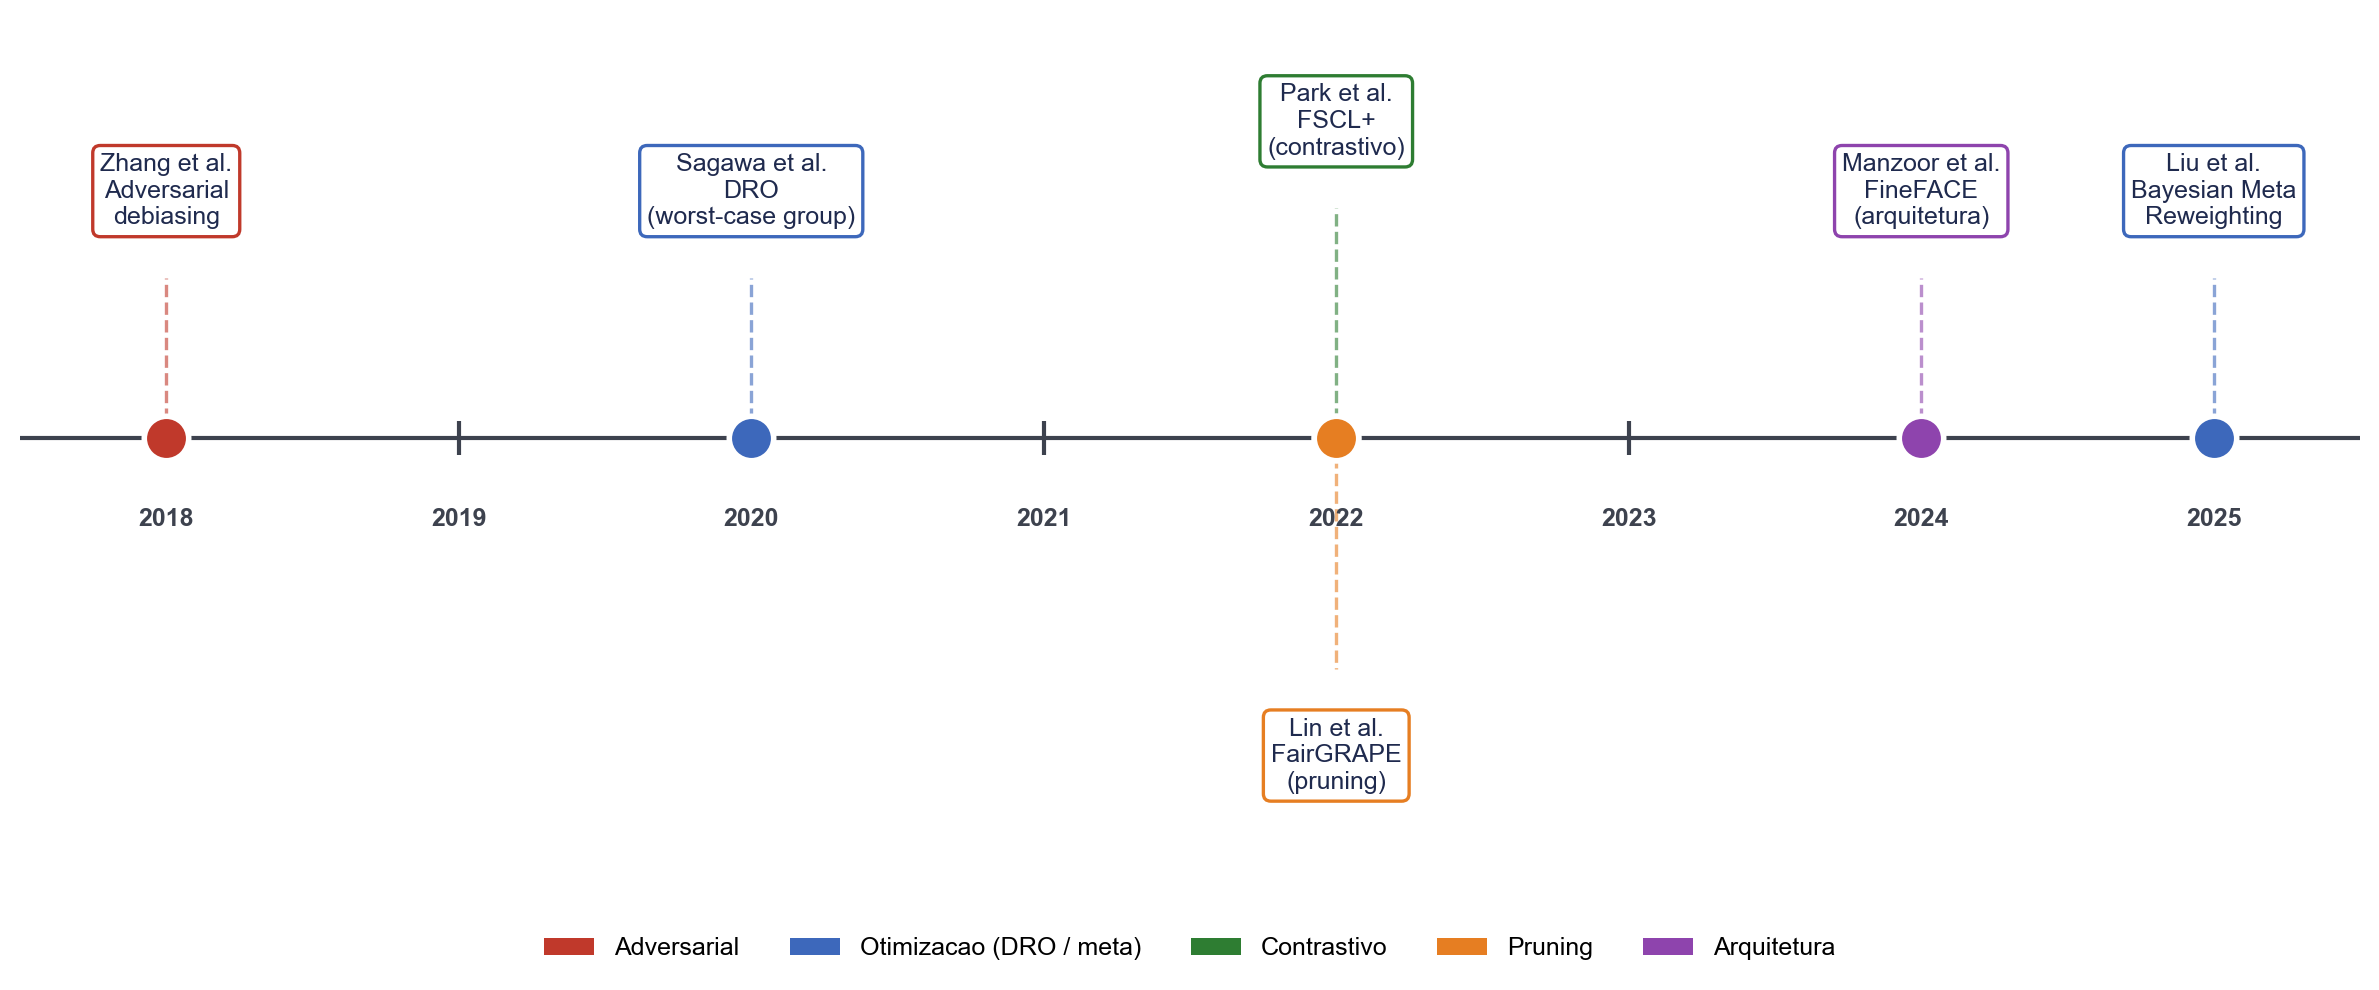
\includegraphics[width=14cm]{images/fig_timeline_mitigacoes.png}
\\ \small Fonte: Autoria própria, com base nas publicações originais de \citeonline{zhang2018mitigating}, \citeonline{sagawa2020distribution}, \citeonline{park2022fair}, \citeonline{lin2022fairgrape}, \citeonline{manzoor2024fineface} e \citeonline{liu2025component}.
\label{fig:timeline-mitigacoes}
\end{figure}

\section{Vision-Language Models}
\label{sec:rl_vlm}

Uma terceira frente emergiu com os \textbf{\emph{Vision-Language Models} (VLMs)}, arquiteturas multimodais capazes de processar simultaneamente imagens e linguagem natural, treinadas em corpora massivos de pares imagem--texto extraídos da \emph{web}. Modelos como CLIP, PaliGemma e LLaVA reformularam tarefas tradicionais de visão computacional em interfaces baseadas em prompts textuais, o que abriu novos caminhos também para o problema de classificação racial.

\citeonline{aldahoul2024exploring} reformularam a classificação racial como \emph{Visual Question Answering} (VQA) --- paradigma em que o modelo recebe uma imagem e uma pergunta em linguagem natural (por exemplo, ``qual é a categoria racial mais provável desta face?'') e responde textualmente --- executado sobre o PaliGemma em regime \emph{fine-tuned}, isto é, ajustado especificamente para a tarefa-alvo. O sistema resultante, denominado FaceScanPaliGemma, atinge o estado da arte atual sobre o FairFace, com 75,7\,\% de acurácia agregada. Para o problema específico de \emph{fairness} em VLMs, \citeonline{luo2024fairclip}, em publicação na conferência CVPR, propuseram o FairCLIP, primeiro dataset \emph{vision-language fair} do domínio médico, introduzindo procedimento de treinamento que penaliza divergências de distribuição entre grupos demográficos por meio da \emph{distância de Sinkhorn} --- métrica de \emph{Optimal Transport} regularizada, computacionalmente tratável e diferenciável, adequada como termo de perda em treinamento de redes profundas. Trabalhos subsequentes como o FairerCLIP~\cite{dehdashtian2024fairerclip}, o BendVLM~\cite{gerych2024bendvlm} e o \emph{debiasing via neural interventions}~\cite{debiasing2025debiasing} oferecem variações metodológicas relevantes, focadas em intervenções sobre o espaço latente do modelo.

Os VLMs trouxeram, em média, desempenho agregado superior, mas simultaneamente introduziram \textbf{novas formas de viés herdadas do corpus de pré-treinamento}. Evidência empírica em escala é oferecida pelo \emph{benchmark} GRAS~\cite{malik2025ask}, que aplicou 2,5 milhões de \emph{queries} de \emph{Visual Question Answering} sobre cem traços de personalidade a cinco VLMs estado da arte, cobrindo os eixos gênero, raça, idade e tom de pele (Monk Skin Tone). Os autores propõem o \emph{GRAS Bias Score}, métrica interpretável no intervalo $[0, 100]$ em que zero representa o ideal de ausência total de viés estatisticamente significativo. O modelo menos enviesado avaliado (\emph{llava-1.5-7b}) obtém pontuação 98, e os demais atingem 99, com diferenças estatisticamente significativas entre grupos demográficos em pelo menos 95 dos 100 traços avaliados. Este achado reforça a observação central da revisão: aumentos de escala e de sofisticação arquitetural não implicam, por si só, mitigação de disparidade demográfica.

A comparação direta de desempenho por raça entre o \emph{baseline} canônico ResNet-34 e o estado da arte VLM (FaceScanPaliGemma) evidencia visualmente essa persistência do gap Latinx, conforme sintetiza a Figura~\ref{fig:f1-sota-comparativo}.

\begin{figure}[htbp]
\centering
\caption{Desempenho por classe racial no FairFace: \emph{baseline} ResNet-34 (2021) \emph{versus} FaceScanPaliGemma (2024).}
\centering
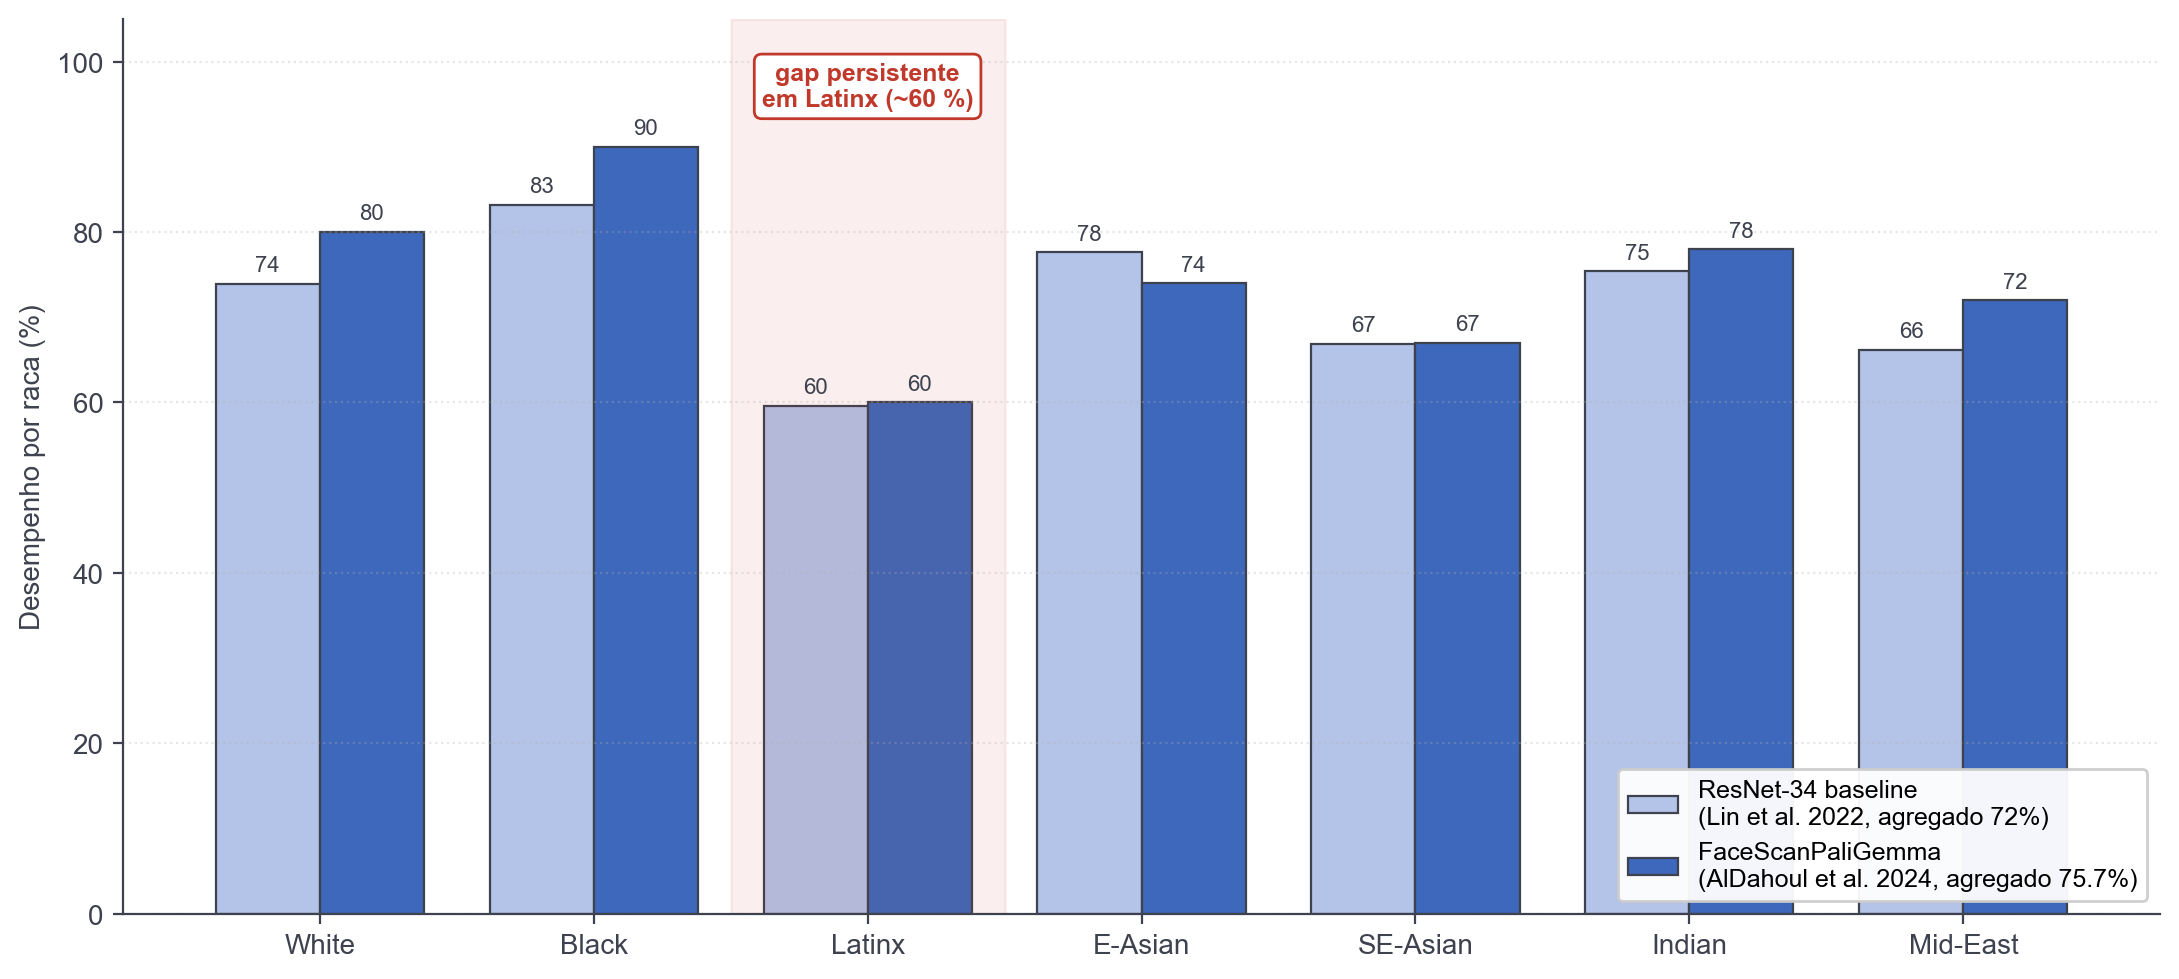
\includegraphics[width=14cm]{images/fig_f1_sota_comparativo.png}
\\ \small Fonte: Autoria própria, com dados extraídos de \citeonline{lin2022fairgrape} (Tabela 2, \emph{baseline} ResNet-34) e de \citeonline{aldahoul2024exploring} (Tabela 16, FaceScanPaliGemma \emph{7-class}).
\label{fig:f1-sota-comparativo}
\end{figure}

\section{Tom de pele como dimensão auditável}
\label{sec:rl_skintone}

Desde o estudo seminal \emph{Gender Shades}~\cite{buolamwini2018gender}, o \textbf{tom de pele} tem sido proposto na literatura como dimensão alternativa de auditoria de \emph{fairness}, mais estável conceitualmente que a categoria racial nominal. A justificativa é epistemológica: enquanto a raça é uma construção sociopolítica cuja definição varia por contexto histórico e cultural, o tom de pele é uma propriedade fenotípica mensurável de forma reproduzível a partir da própria imagem, funcionando como sinal objetivo para auditoria automatizada.

A primeira escala amplamente adotada foi a de \citeonline{fitzpatrick1988validity}, originalmente desenvolvida na dermatologia para determinar tolerância à fototerapia com radiação ultravioleta. A escala Fitzpatrick classifica a pele em seis fototipos (I a VI) segundo reatividade à exposição solar, e foi transferida à pesquisa de \emph{fairness} em inteligência artificial apesar de seu \textbf{viés caucasiano-cêntrico documentado} --- os quatro primeiros fototipos (I a IV) discriminam finamente peles claras, ao passo que apenas dois fototipos (V e VI) cobrem todo o espectro de peles escuras, produzindo resolução assimétrica indesejável para auditoria demográfica.

Em resposta a essa limitação, \citeonline{schumann2023consensus} estabeleceram formalmente, em 2023, a \textbf{Monk Skin Tone Scale} (MST), escala de dez pontos desenvolvida em parceria entre o sociólogo Ellis Monk (Universidade de Harvard) e a equipe de \emph{Responsible AI} do Google, projetada especificamente para auditoria de \emph{fairness} em sistemas de inteligência artificial. Ao distribuir os dez pontos de forma perceptualmente mais uniforme ao longo do espectro de tons, a MST oferece resolução simétrica entre peles claras e escuras, o que a consolidou como padrão moderno de referência. A Figura~\ref{fig:fitzpatrick-mst} contrasta visualmente as duas escalas, evidenciando a assimetria de Fitzpatrick e a distribuição simétrica da MST.

\begin{figure}[htbp]
\centering
\caption{Comparação entre as escalas Fitzpatrick (1988) e Monk Skin Tone (2023).}
\centering
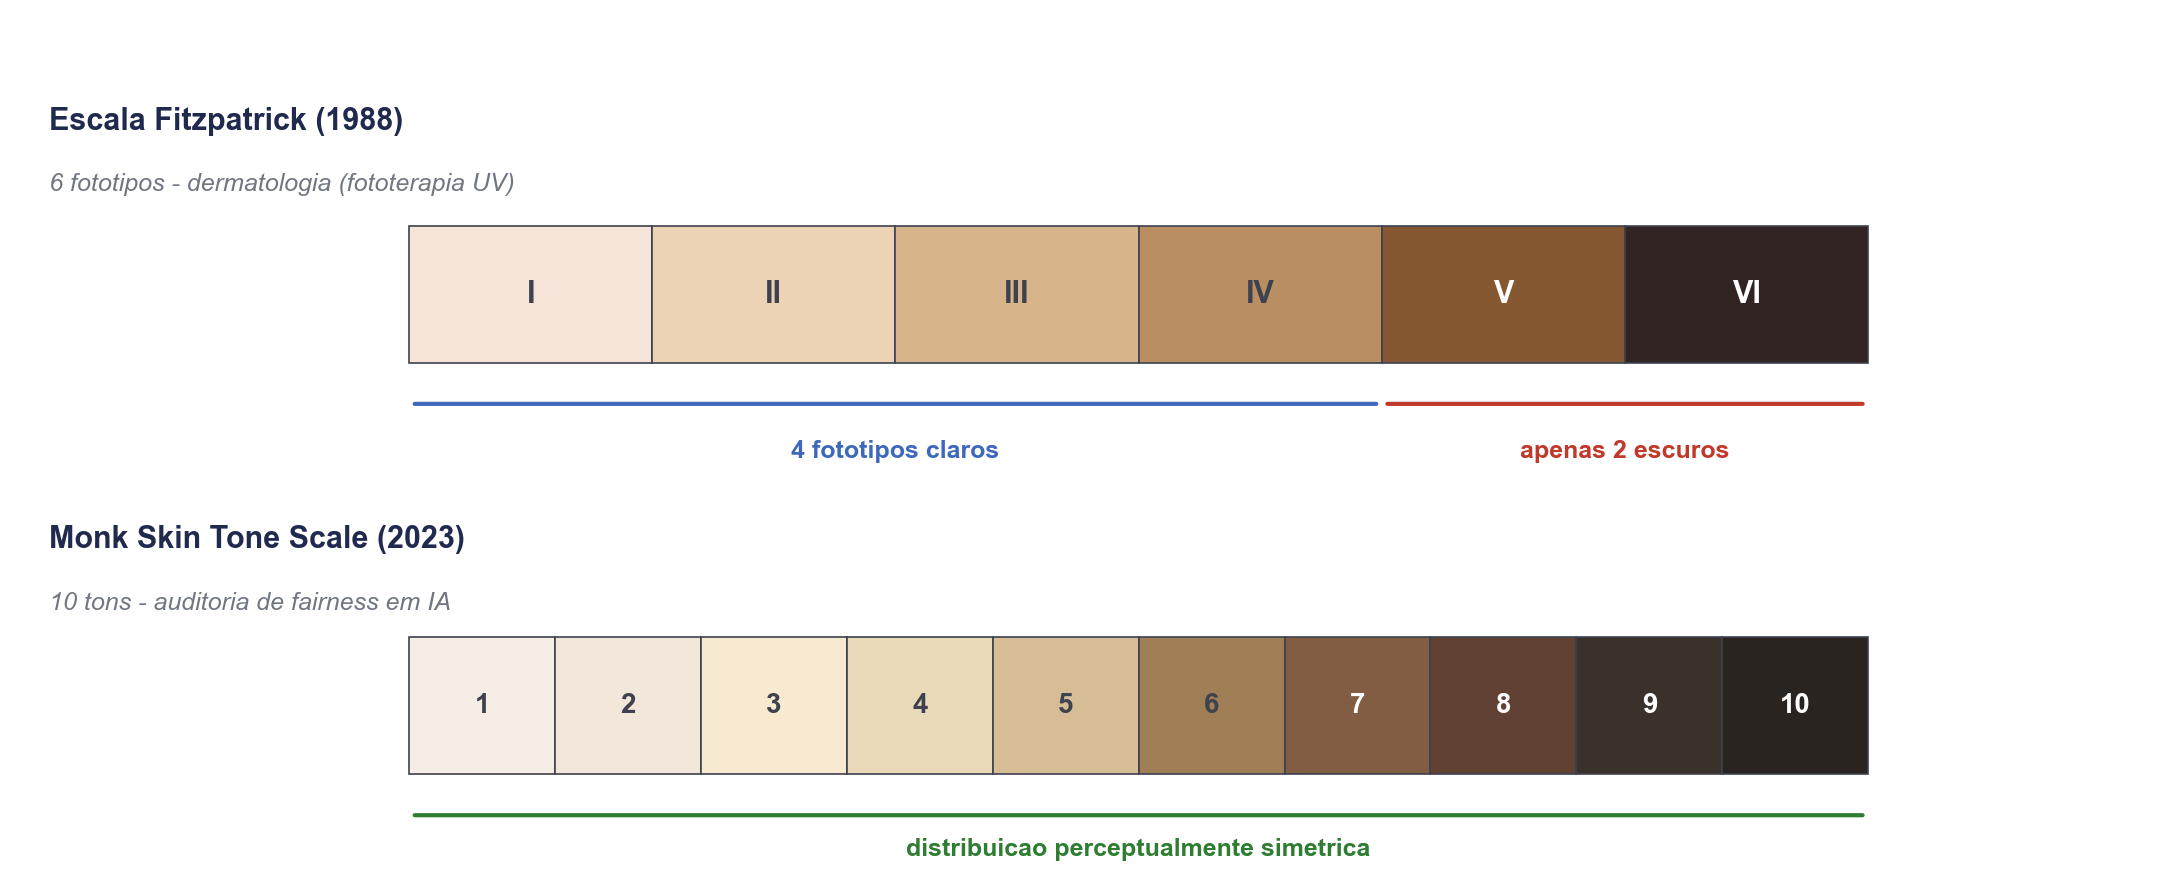
\includegraphics[width=14cm]{images/fig_fitzpatrick_vs_mst.png}
\\ \small Fonte: Autoria própria, com cores oficiais da Monk Skin Tone Scale publicadas em \emph{skintone.google}~\cite{schumann2023consensus} e cores Fitzpatrick derivadas de referências dermatológicas públicas com base em \citeonline{fitzpatrick1988validity}.
\label{fig:fitzpatrick-mst}
\end{figure}

Em 2026, \citeonline{matias2026large} introduziram o \textbf{SkinToneNet}, um classificador MST em larga escala baseado na arquitetura Vision Transformer Small (ViT-S), ajustada (\emph{fine-tuned}) sobre o dataset \emph{Skin Tone in the Wild} (STW), composto por 42.313 imagens de 3.564 indivíduos. O SkinToneNet atinge estado da arte em regime \emph{cross-domain}, isto é, quando avaliado em datasets distintos daquele utilizado no treinamento. Este modelo é adotado como insumo pré-treinado na Etapa~1 do pipeline proposto (Seção~\ref{sec:pipeline}), acompanhado de \emph{sensitivity analysis} a classificadores MST alternativos como salvaguarda contra propagação de viés herdado.

Uma frente emergente de crítica questiona, contudo, o próprio paradigma de rotulagem \textbf{discreta} do tom de pele. \citeonline{neto2025balancing}, em contribuição recente, argumentam que a fragmentação do espectro fenotípico em classes discretas --- seja MST-10, Fitzpatrick-6 ou categorias raciais nominais --- impõe limite estrutural à mitigação de viés, uma vez que identidades dentro de uma mesma categoria não contribuem igualmente ao balanceamento demográfico do dataset. Os autores propõem \emph{rótulos demográficos contínuos}, obtidos como grau de pertencimento produzido por um classificador de etnia treinado sobre um sistema de \emph{face recognition} estado da arte, demonstrando que modelos treinados com balanceamento no espaço contínuo superam consistentemente aqueles treinados no espaço discreto. A presente pesquisa mantém a MST discreta como escolha metodológica principal, por sua consolidação como padrão de auditoria desde 2023 e pela ausência de classificadores contínuos publicamente disponíveis e amplamente validados em 2026, mas registra a linha contínua como direção natural de trabalho futuro, discutida no Capítulo~\ref{chapter:cronograma}.


\section{Heterogeneidade fenotípica intra-categorial}
\label{sec:rl_latinx}

A persistência do F1 na faixa de 60\,\% para a categoria \emph{Latinx} no estado da arte, apesar do balanceamento amostral e das técnicas de mitigação algorítmica avançada revistas nas seções anteriores, sugere a existência de um limite estrutural que a intervenção puramente computacional não é capaz de ultrapassar. Essa observação motivou a incorporação a esta pesquisa de uma frente teórica adicional --- oriunda de disciplinas externas à ciência da computação --- segundo a qual \textbf{a categoria Latinx/Hispanic, tal como operacionalizada no FairFace, mascara heterogeneidade fenotípica interna substantiva}. Três aportes disciplinares independentes convergem para essa hipótese:

\begin{itemize}
\item \textbf{Antropologia biológica.} \citeonline{telles2014pigmentocrac}, através do projeto PERLA (\emph{Project on Ethnicity and Race in Latin America}), documentou pigmentocracia em quatro países latino-americanos --- Brasil, Colômbia, México e Peru ---, mostrando que tom de pele opera como dimensão social distinta da categoria racial, e que a variabilidade fenotípica intra-país é maior que a variabilidade entre países.

\item \textbf{Genética populacional.} \citeonline{bryc2015genetic}, em estudo publicado no \emph{American Journal of Human Genetics} com amostra de 162.721 indivíduos, evidenciou que Latinos exibem composição altamente variável de ancestralidade Native American, European e African, com desvios-padrão intra-categoria comparáveis à variação entre outros grupos.

\item \textbf{Sociologia identitária.} O Pew Research Center~\cite{lopez2017hispanic} documentou que a identidade Hispanic declina de 97\,\% para 50\,\% ao longo de quatro gerações nos Estados Unidos, caracterizando a categoria como sociopolítica e fluida, e não como fenotípica ou biológica estável.
\end{itemize}

Essa triangulação teórica interdisciplinar sustenta uma das hipóteses formalizadas no Capítulo~\ref{chapter:objetivos}, segundo a qual a categoria Latinx no FairFace exibe dispersão ampla ao longo da escala Monk Skin Tone (cobertura de cinco ou mais das dez classes), oferecendo fundamentação empírica externa à ciência da computação para o diagnóstico de heterogeneidade estrutural que motiva o pipeline proposto. Trata-se de deslocamento epistemológico deliberado: a hipótese passa a ser testada com evidência produzida por antropologia, genética e sociologia, e não apenas por métricas internas ao próprio benchmark computacional.

\section{Fair representation learning}
\label{sec:rl_fairrep}

Parte da literatura recente contesta o uso do tom de pele como principal \emph{driver} explicativo da disparidade racial. A contribuição mais relevante nessa direção é a de \citeonline{pangelinan2023exploring}, que sustenta que o gap racial em \emph{face recognition} é primariamente explicado por diferenças de \emph{pixel information} --- a fração de área útil da face contida na imagem, obtida por segmentação semântica com a rede BiSeNet ---, colocando o tom de pele em segundo plano na hierarquia causal. A presente pesquisa incorpora essa crítica de forma explícita sob duas formas complementares: primeiro, mediante controle de \emph{pixel information} como \emph{confounder} --- variável correlacionada tanto com o atributo sensível quanto com o desempenho --- na Etapa~5 do pipeline (Seção~\ref{sec:pipeline}); segundo, por meio de uma hipótese formalizada no Capítulo~\ref{chapter:objetivos} desenhada como teste direto da tese de \citeauthoronline{pangelinan2023exploring}. A inclusão explícita da refutação é decisão metodológica deliberada: fortalece a validade externa do resultado positivo, caso obtido, e o expõe honestamente à possibilidade de refutação, caso não obtido.

Em uma linhagem teórica complementar, \citeonline{zemel2013learning} inauguraram, com o paradigma de \emph{Learning Fair Representations}, a ideia de \textbf{representações intermediárias com propriedade de \emph{fairness}} --- vetores latentes cuja construção incorpora restrições explícitas de equidade e que preservam informação útil para a tarefa-alvo enquanto suprimem informação sobre o atributo sensível. O trabalho recebeu, em 2023, o \emph{Test-of-Time Award} da ICML, prêmio concedido pela conferência a artigos cujo impacto sustentado ao longo de uma década é reconhecido pela comunidade.

\citeonline{madras2018learning} estenderam o paradigma com o LAFTR (\emph{Learning Adversarially Fair and Transferable Representations}), demonstrando teoricamente que se a representação intermediária $Z$ satisfaz uma propriedade de \emph{fairness} em uma tarefa, então qualquer classificador \emph{downstream} treinado sobre $Z$ herda um limite superior formal para a violação daquela propriedade. Trata-se de garantia teórica de \emph{transferência de fairness} entre tarefas. \citeonline{aguirre2023transferring} corroboraram empiricamente essa transferência no domínio de Processamento de Linguagem Natural (NLP), em arquitetura \emph{multi-task} (múltiplas tarefas treinadas conjuntamente), obtendo reduções relativas de quinze a quarenta e quatro por cento na métrica $\varepsilon$-DEO (\emph{$\varepsilon$-Differential Equalized Odds}, medida da maior violação de \emph{Equalized Odds} entre grupos) sem perda de F1. A definição formal de \emph{Equal Opportunity} e de \emph{Equalized Odds} que estrutura toda essa literatura foi estabelecida por \citeonline{hardt2016equality} e é retomada formalmente na Seção~\ref{sec:rl_metricas} deste capítulo.

\section{Arquiteturas \emph{backbone}}
\label{sec:rl_backbones}

A escolha do \emph{backbone} --- rede neural responsável por produzir representações intermediárias das imagens antes da camada final de classificação --- é decisão metodológica central em qualquer sistema de reconhecimento facial, e impacta diretamente tanto o desempenho agregado quanto o comportamento de \emph{fairness} entre subgrupos demográficos. Do ponto de vista computacional, a literatura contemporânea de visão computacional organiza-se em torno de \textbf{dois paradigmas complementares}: o paradigma \emph{convolucional}, que opera por meio de filtros locais e estrutura hierárquica, e o paradigma \emph{baseado em atenção}, que opera por meio de \emph{self-attention} sobre representações tokenizadas da imagem. Esta seção percorre ambos os paradigmas para contextualizar a escolha metodológica formalizada no Capítulo~\ref{chapter:metodologia}.

\subsection{Paradigma convolucional}
\label{sec:rl_backbones_conv}

O paradigma convolucional é o mais antigo e o dominante em visão computacional. Desde LeNet, AlexNet e VGG, as \emph{Convolutional Neural Networks} (CNNs) profundas foram sucessivamente aperfeiçoadas até que, em 2015, a família ResNet introduziu o mecanismo de \emph{conexões residuais} que viabilizou o treinamento estável de redes com dezenas a centenas de camadas, tornando-se o padrão de \emph{backbone} para a década seguinte. No contexto da literatura de \emph{fairness} facial revisada, a variante ResNet-34 foi adotada por \citeonline{karkkainen2021fairface} como \emph{baseline} original do FairFace e, consequentemente, tornou-se referência recorrente ao longo do corpus: foi retomada por \citeonline{lin2022fairgrape} como \emph{baseline} de comparação do FairGRAPE e por \citeonline{aldahoul2024exploring} como controle contra o qual o FaceScanPaliGemma foi comparado.

A face contemporânea deste mesmo paradigma é a família \textbf{ConvNeXt}, proposta por \citeonline{liu2022convnet}. Sua contribuição é a \emph{modernização} sistemática da linha ResNet a partir de escolhas de design importadas dos Vision Transformers --- sem, contudo, adotar qualquer módulo de atenção. Os autores partem de uma ResNet-50 tradicional e aplicam, de forma incremental, cinco classes de modernizações: (i) redesenho macro (razão de estágios $[3, 3, 9, 3]$ e \emph{stem} tipo \emph{patchify}); (ii) adoção de \emph{depthwise convolutions} à ResNeXt; (iii) \emph{inverted bottleneck}; (iv) \emph{large kernel sizes} ($7 \times 7$); e (v) micro-design (\emph{LayerNorm} em substituição a \emph{BatchNorm}, ativação \emph{GELU}, redução do número de camadas de ativação e normalização). A Figura~\ref{fig:convnext-teaser}, reproduzida do repositório oficial dos autores, evidencia dois pontos centrais: à esquerda, a comparação de acurácia \emph{Top-1} em ImageNet-1K entre ResNet, DeiT, Swin Transformer, ViT e ConvNeXt em dois regimes (treino direto e \emph{pré-treino} em ImageNet-22K), mostrando que o ConvNeXt supera consistentemente as arquiteturas contemporâneas sob o mesmo orçamento de FLOPs; à direita, a comparação lado a lado dos blocos internos das três arquiteturas (Swin, ResNet e ConvNeXt), tornando visualmente evidente que o bloco ConvNeXt permanece \emph{puramente convolucional} (sem \emph{Multi-Head Self-Attention}), diferentemente do bloco Swin.

\begin{figure}[htbp]
\centering
\caption{Comparação entre \emph{backbones} contemporâneos: acurácia \emph{Top-1} em ImageNet-1K (esquerda) e estrutura dos blocos internos de Swin, ResNet e ConvNeXt (direita).}
\centering
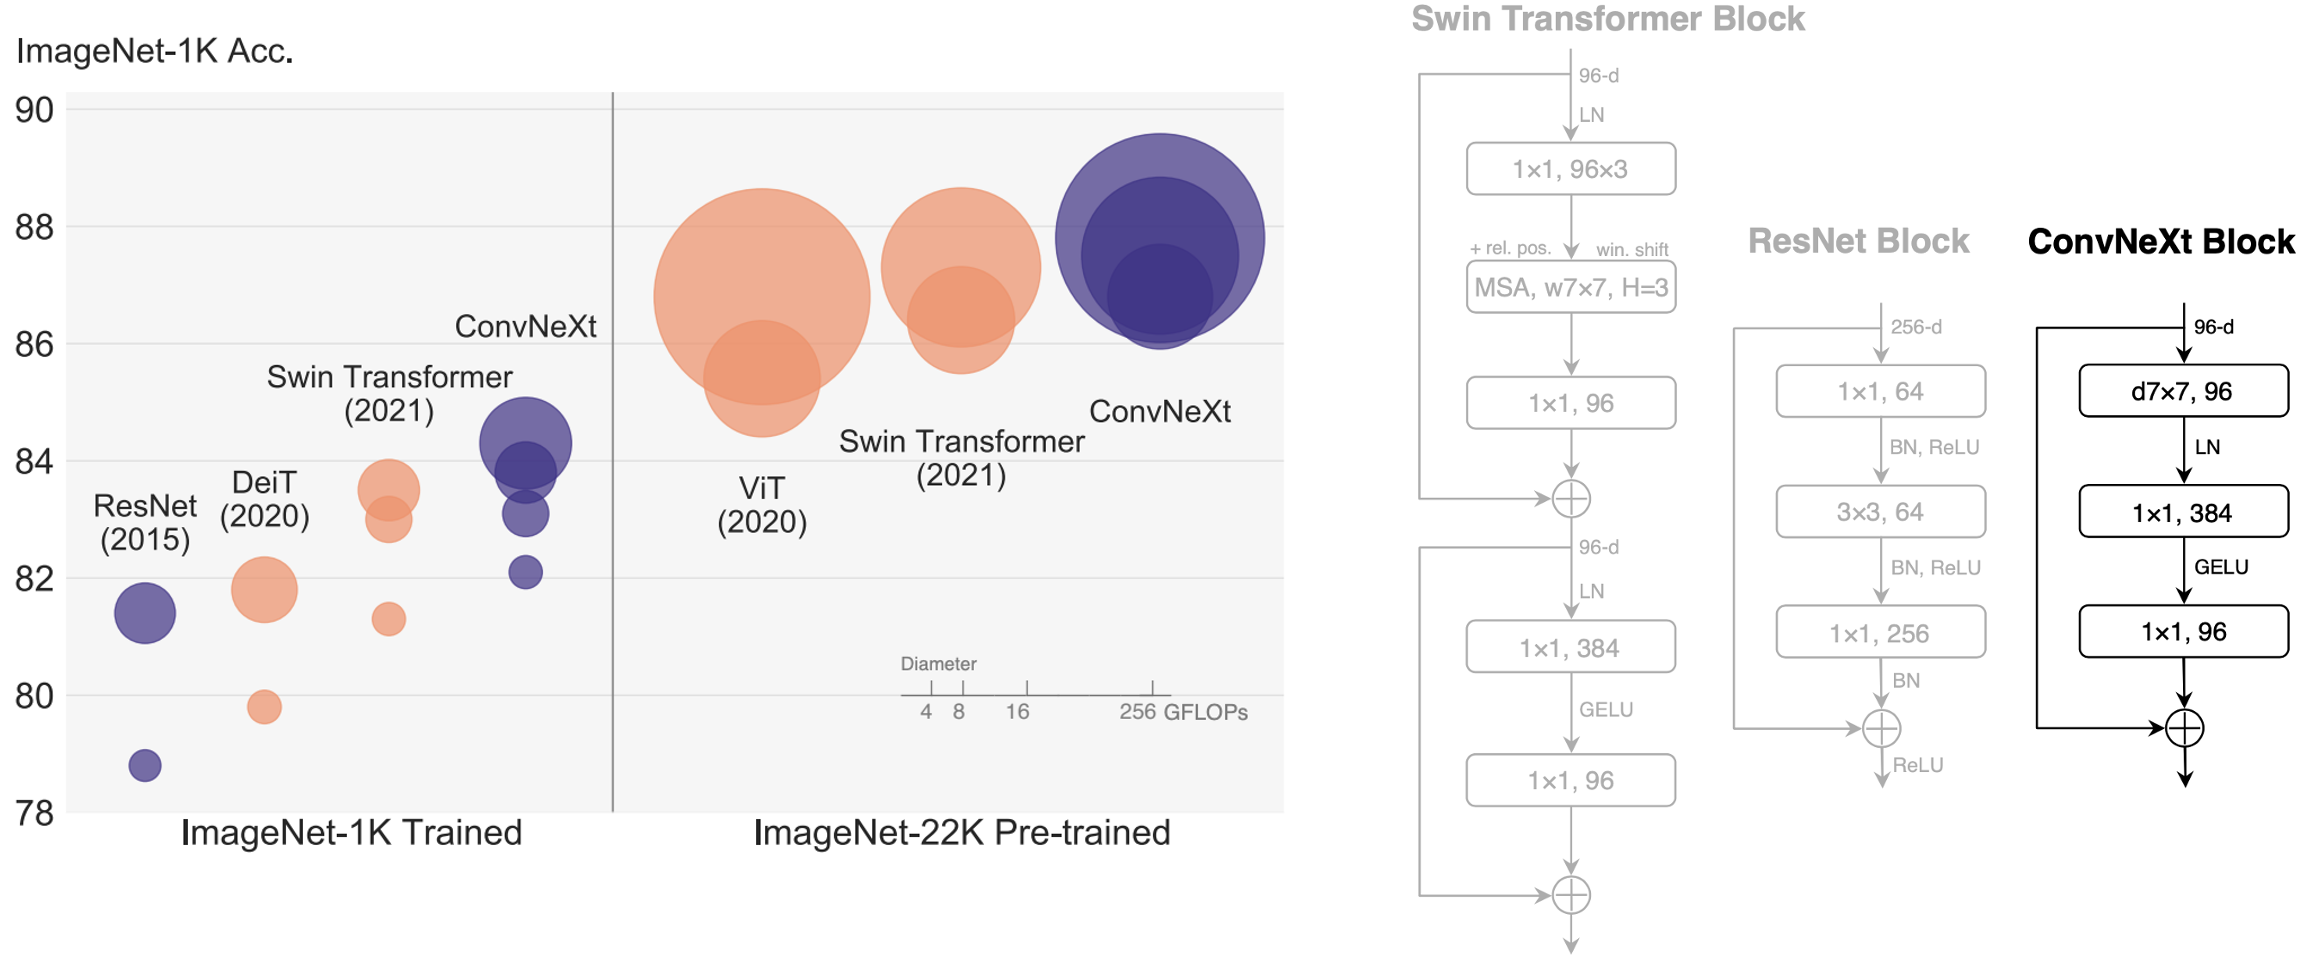
\includegraphics[width=15cm]{images/fig_convnext_teaser_meta.png}
\\ \small Fonte: \citeonline{liu2022convnet} --- teaser oficial do repositório \emph{facebookresearch/ConvNeXt}, disponível em \emph{github.com/facebookresearch/ConvNeXt}. Reprodução com finalidade acadêmica sob os termos de uso permitido para citação.
\label{fig:convnext-teaser}
\end{figure}

\subsection{Paradigma de atenção}
\label{sec:rl_backbones_vit}

O paradigma baseado em atenção emergiu em visão computacional em 2020, com a proposta dos \emph{Vision Transformers} (ViTs) --- aplicação do mecanismo de \emph{self-attention} originalmente desenvolvido para processamento de linguagem natural ao domínio visual, por meio da tokenização de imagens em \emph{patches} tratados como sequências. Variantes hierárquicas subsequentes, como o Swin Transformer, incorporaram estrutura \emph{multi-scale} para reduzir custo computacional e ampliar aplicabilidade em tarefas de detecção e segmentação.

No corpus revisado, ViTs aparecem tanto em propostas específicas de \emph{fairness} arquitetural --- como o FairViT de \citeonline{tian2024fairvit} --- quanto como \emph{backbone} de referência para classificação de tom de pele, notadamente no SkinToneNet~\cite{matias2026large}, que adota Vision Transformer Small (ViT-S). Contudo, ViTs apresentam três limitações relevantes em relação a esta pesquisa: (i) exigência de datasets massivos de pré-treinamento para atingir desempenho competitivo em regime de \emph{fine-tuning} sobre datasets de escala média como o FairFace; (ii) custo computacional elevado em inferência; e (iii) natureza \emph{non-hierarchical} da variante padrão, o que dificulta a inserção de mecanismos de \emph{conditioning} como FiLM originalmente projetados para redes convolucionais em quatro estágios.

\subsection{Justificativa da escolha}
\label{sec:rl_backbones_escolha}

A escolha metodológica adotada neste trabalho é o ConvNeXt-T --- a variante \emph{Tiny} (aproximadamente 28 milhões de parâmetros) da família ConvNeXt. Trata-se, conforme discutido na Seção~\ref{sec:rl_backbones_conv}, de uma CNN moderna dentro do paradigma convolucional, e não de uma alternativa paradigmática a ele. Essa posição é conveniente porque permite manter a comparabilidade estrutural direta com o \emph{baseline} canônico ResNet-34 --- ambos são CNNs hierárquicas, permitindo isolar o efeito da modernização arquitetural sem confundi-lo com uma mudança de paradigma computacional.

O impacto do \emph{backbone} sobre o comportamento de \emph{fairness} não é neutro: \citeonline{dooley2023rethinking}, por meio de \emph{Neural Architecture Search}, demonstraram empiricamente que decisões arquiteturais específicas afetam diretamente o padrão de disparidade demográfica observado, reforçando a exigência metodológica de justificar formalmente a escolha do \emph{backbone} em contextos sensíveis a \emph{fairness}. A justificativa detalhada da adoção do ConvNeXt-T --- que considera paridade competitiva com ViTs, estabilidade de treinamento em \emph{fine-tuning}, compatibilidade nativa com o mecanismo FiLM e comparabilidade com o \emph{baseline} canônico ResNet-34 --- é apresentada na Seção~\ref{sec:backbone} do Capítulo de Metodologia.


\section{Métricas de \emph{fairness}}
\label{sec:rl_metricas}

Toda a literatura revisada nas seções anteriores depende de definições formais para a noção de \emph{fairness} algorítmico. A ausência de uma métrica única e universalmente aceita é, ela própria, uma característica estrutural do campo, com consequência metodológica direta para o desenho experimental proposto nesta dissertação.

\subsection{Definições canônicas em nível de grupo}
\label{sec:rl_metricas_defs}

Seja um classificador $h: \mathcal{X} \to \mathcal{Y}$, um atributo sensível $A$ (raça, no contexto deste trabalho), o rótulo verdadeiro $Y$ e a predição $\widehat{Y} = h(X)$. As três definições \emph{group-level} mais adotadas na literatura de \emph{fairness} são:

\begin{itemize}
\item \textbf{Paridade Demográfica (\emph{Demographic Parity} ou \emph{Statistical Parity})}, formalizada por \citeonline{dwork2012fairness}, exige que $P(\widehat{Y} = 1 \mid A = a) = P(\widehat{Y} = 1 \mid A = b)$ para quaisquer grupos $a, b$: a taxa de predições positivas deve ser independente do atributo sensível. É historicamente a métrica mais antiga, mas ignora a distribuição real de $Y$ entre grupos, podendo penalizar classificadores acurados quando as taxas-base diferem entre populações --- limitação criticada pelos próprios autores como motivação para a formulação alternativa de \emph{individual fairness}.

\item \textbf{Igualdade de Oportunidade (\emph{Equal Opportunity})}, formalizada por \citeonline{hardt2016equality}, exige que $P(\widehat{Y} = 1 \mid A = a, Y = 1) = P(\widehat{Y} = 1 \mid A = b, Y = 1)$, ou seja, igualdade das taxas de verdadeiro-positivo entre grupos. É adequada a contextos em que o custo do falso-negativo é o problema central.

\item \textbf{Equalização de Chances (\emph{Equalized Odds})}, também de \citeonline{hardt2016equality}, é extensão mais restritiva que exige simultaneamente a igualdade das taxas de verdadeiro-positivo \emph{e} de falso-positivo entre grupos.
\end{itemize}

Além destas três definições, a literatura de mitigação revisada emprega recorrentemente três métricas derivadas: (i) \emph{Disparity Ratio} (DR), razão entre o desempenho do melhor e do pior grupo demográfico; (ii) \emph{worst-class F1}, F1 do grupo mais penalizado, adotado como função-objetivo por \citeonline{sagawa2020distribution}; e (iii) F1 \emph{macro} agregado, adotado por \citeonline{aldahoul2024exploring} sobre o FairFace \emph{7-class}. Cada métrica captura uma dimensão distinta da equidade, e nenhuma isoladamente oferece diagnóstico completo do desempenho de um classificador sob restrição de \emph{fairness}.

\subsection{O Teorema da Impossibilidade}
\label{sec:rl_metricas_impossibilidade}

O resultado formal mais influente da literatura contemporânea de \emph{fairness} algorítmico é o Teorema da Impossibilidade, demonstrado por \citeonline{kleinberg2017inherent}. Os autores provam que três critérios naturais de equidade --- calibração entre grupos, balanceamento das taxas de falso-positivo e balanceamento das taxas de falso-negativo --- \textbf{não podem ser satisfeitos simultaneamente} por um mesmo classificador, exceto em dois casos triviais: predições perfeitas ou taxas-base idênticas entre grupos.

A consequência metodológica é direta e incontornável: qualquer intervenção que otimize uma das definições formais de \emph{fairness} violará necessariamente ao menos uma outra. Não existe, portanto, \emph{classificador universalmente justo}; existem, apenas, classificadores que satisfazem trade-offs explícitos entre definições concorrentes. Esta observação motiva o princípio metodológico de \textbf{triangulação de métricas} adotado nesta pesquisa.

\subsection{Adaptações multi-classe}
\label{sec:rl_metricas_multiclasse}

Todas as definições formais apresentadas foram originalmente formuladas em contexto binário ($\mathcal{Y} = \{0, 1\}$). Para a classificação racial \emph{multi-classe} do FairFace (sete categorias), a literatura revisada \textbf{não converge em um protocolo único de adaptação}: algumas abordagens reduzem o problema a agregações binárias por classe (\emph{one-vs-rest}), outras empregam extensões macro/micro, e outras ainda avaliam apenas o pior subgrupo sem \emph{cross-tabulation} sistemática. Esta fragmentação é retomada explicitamente como a Lacuna 5 na Seção~\ref{sec:rl_gaps} e motiva a proposta metodológica de triangulação apresentada na Seção~\ref{sec:metricas} do Capítulo de Metodologia, na qual três métricas complementares são reportadas simultaneamente para cada configuração experimental como salvaguarda operacional contra o Teorema da Impossibilidade.

Cabe registrar que, em 2024, o esforço internacional de padronização convergiu com a publicação da norma \textbf{ISO/IEC 19795-10:2024}~\cite{iso2024biometric}, que estabelece diretrizes formais para o reporte de variação de desempenho de sistemas biométricos entre grupos demográficos. A norma consolida, em linguagem regulatória, a prática de triangulação de métricas já emergente na literatura acadêmica revisada, e converge com as obrigações de auditoria de \emph{fairness} estabelecidas pelo \emph{European AI Act} para sistemas biométricos classificados como de alto risco. O protocolo experimental proposto no Capítulo~\ref{chapter:metodologia} adere a essas diretrizes ao reportar sistematicamente desempenho estratificado por grupo racial em três métricas complementares.

\section{Auditoria de datasets e mecanismos de \emph{conditioning}}
\label{sec:rl_arquit}

Paralelamente às frentes teórico-empíricas percorridas até aqui, consolida-se uma \textbf{frente instrumental} organizada em torno de duas classes de ferramentas: procedimentos automatizados de auditoria de datasets e mecanismos arquiteturais de \emph{conditioning}. A primeira classe fornece diagnósticos sobre onde e como o viés se manifesta; a segunda oferece intervenções concretas para incorporar informação auxiliar ao processamento interno das redes.

Na frente de \textbf{auditoria de datasets}, \citeonline{dooley2023rethinking} demonstraram inicialmente, por meio de \emph{Neural Architecture Search} (NAS) --- técnica automatizada de busca no espaço de arquiteturas neurais possíveis ---, que padrões de viés podem estar inerentemente associados a escolhas arquiteturais específicas, e não apenas aos dados de treinamento, o que expande o escopo do problema para o próprio nível do desenho da rede. No ano seguinte, \citeonline{dominguezcatena2024dsap} propuseram o DSAP (\emph{Dataset Similarity via Attribute Proportions}), \emph{framework} unificado que quantifica similaridade entre distribuições de atributos demográficos por meio do \textbf{índice de Renkonen} --- métrica de sobreposição de proporções entre duas distribuições categóricas, historicamente empregada em ecologia para medir similaridade de comunidades e adotada aqui como sinal comparável entre datasets. Já em 2025, \citeonline{lafargue2025fairness} propuseram um \emph{pipeline} de auditoria de \emph{fairness} com testes estatísticos \emph{uncertainty-aware}, isto é, testes que propagam explicitamente a incerteza amostral ao veredito final de disparidade, evitando conclusões precipitadas a partir de subgrupos pouco representados.

Quanto a \textbf{mecanismos arquiteturais de \emph{conditioning}} --- entendidos como técnicas que injetam informação auxiliar diretamente nas representações internas de uma rede neural durante o \emph{forward pass} ---, o marco fundacional é o FiLM (\emph{Feature-wise Linear Modulation}), proposto por \citeonline{perez2018film}: mecanismo \emph{parameter-efficient} (com número de parâmetros adicionais reduzido em relação ao \emph{backbone}) e amplamente adotado em domínios como \emph{Visual Question Answering}, síntese condicional de imagens e robótica. A Figura~\ref{fig:film-conceitual} apresenta o diagrama conceitual do mecanismo, adaptado da formulação original de \citeauthoronline{perez2018film}. Contudo, conforme argumentado na Seção~\ref{sec:rl_gaps}, o FiLM \textbf{ainda não foi testado como mecanismo de mitigação de viés em classificação racial multi-classe} na literatura consultada. Alternativas modernas incluem, também em ordem cronológica, os Vision Transformers \emph{fairness-aware} como o FairViT~\cite{tian2024fairvit} (2024), as abordagens baseadas em \emph{Low-Rank Adaptation} (LoRA)~\cite{sukumaran2024fairlora,bian2025lora} (2024--2025) e o AIM-Fair~\cite{zhao2025aim} (2025). A análise comparativa detalhada dos mecanismos de \emph{conditioning} candidatos é apresentada na próxima seção, e uma das configurações descritas no Capítulo~\ref{chapter:metodologia} (Seção~\ref{sec:ablation}) opera como \emph{ablation} arquitetural direta contra FiLM sobre \emph{embedding} textual do CLIP.

\begin{figure}[htbp]
\centering
\caption{Diagrama conceitual do mecanismo \emph{Feature-wise Linear Modulation} (FiLM).}
\centering
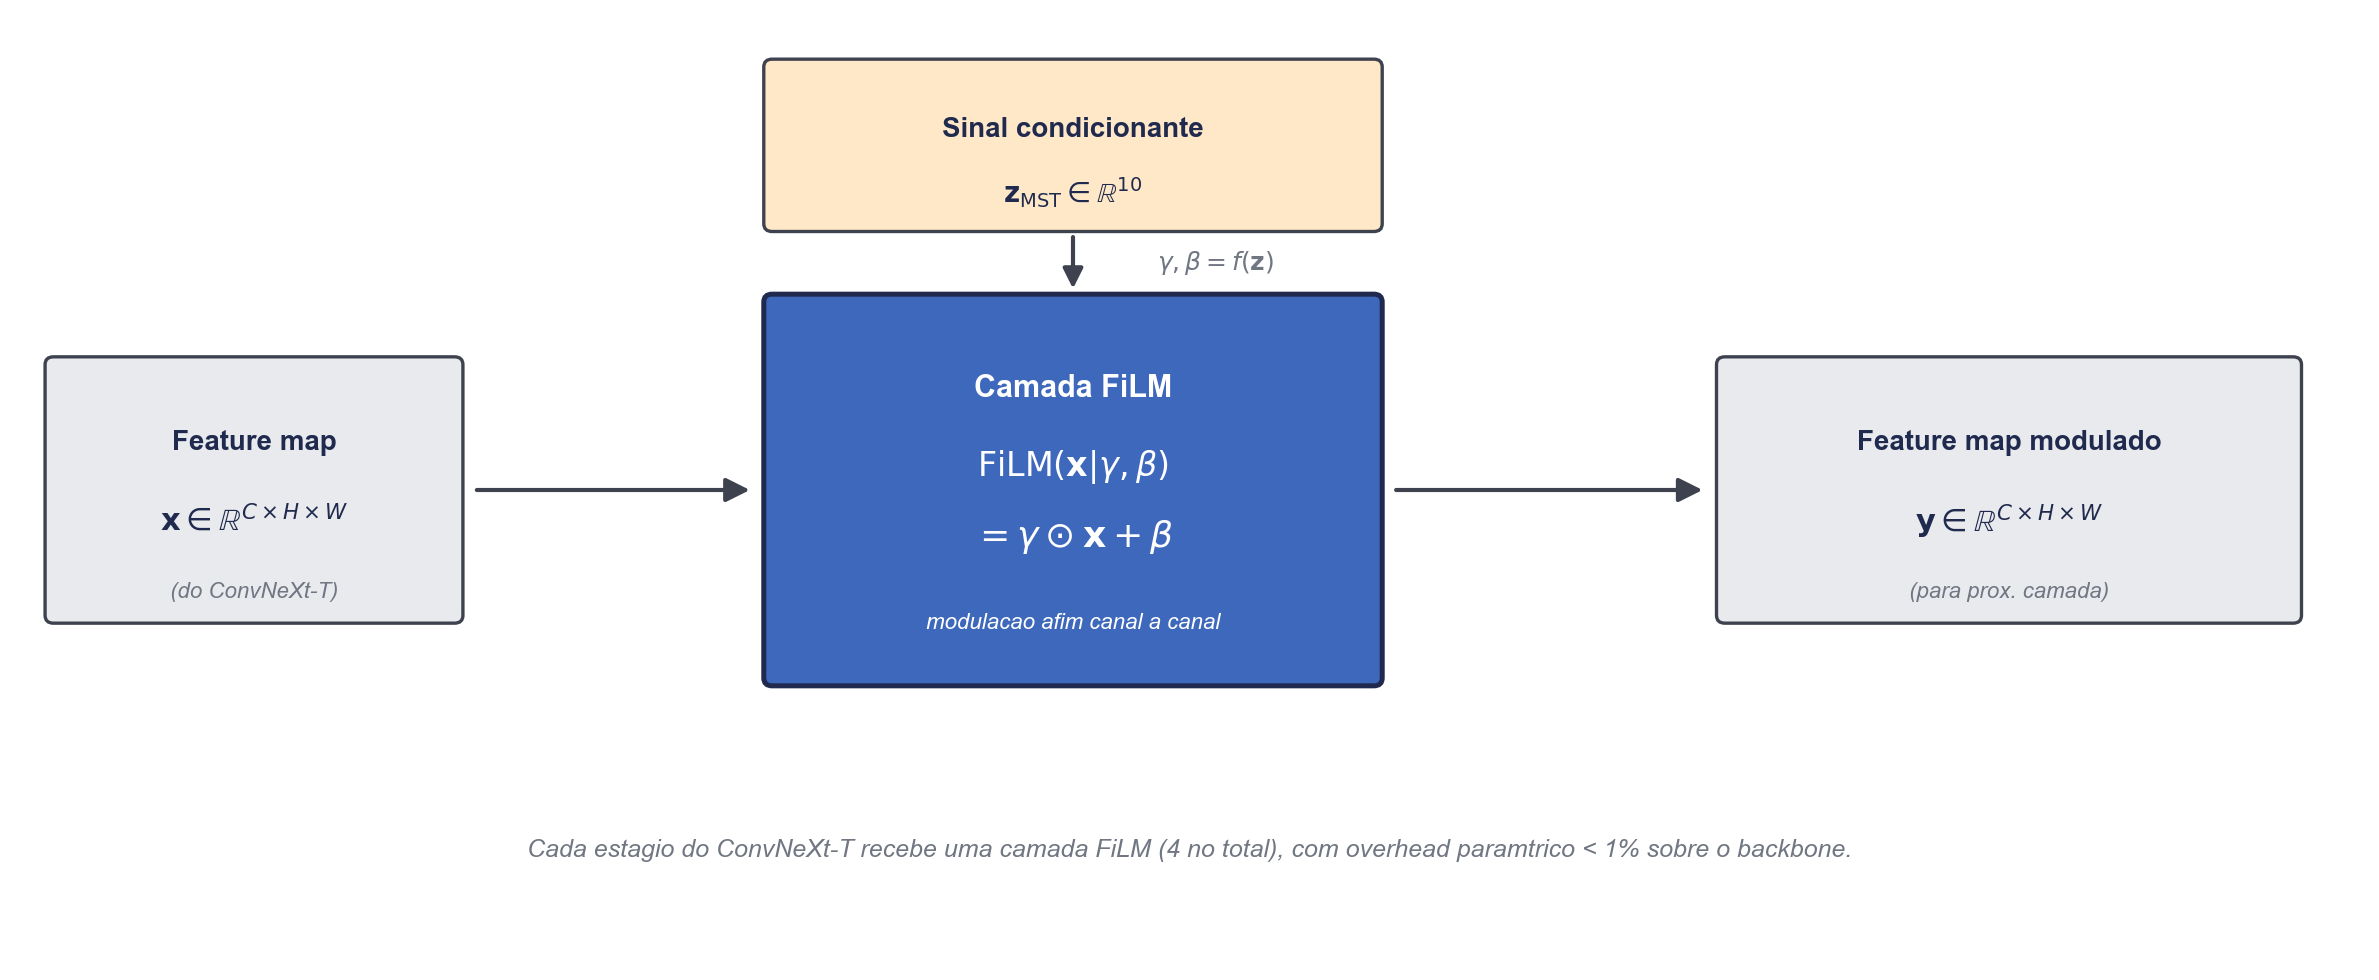
\includegraphics[width=14cm]{images/fig_film_conceitual.png}
\\ \small Fonte: Autoria própria, adaptado da formulação e da representação gráfica originais de \citeonline{perez2018film} (Figura 2 do artigo).
\label{fig:film-conceitual}
\end{figure}

\section{Alternativas de \emph{conditioning}}
\label{sec:rl_conditioning_alt}

A escolha do mecanismo FiLM como linha principal desta pesquisa se fundamenta na avaliação sistemática de oito alternativas de \emph{conditioning} disponíveis na literatura. A Tabela~\ref{tab:cond_alternativas} sintetiza essa análise considerando o cenário específico desta pesquisa: sinal de \emph{conditioning} vetorial de baixa dimensionalidade (vetor Monk Skin Tone de dez classes na saída \emph{softmax} do classificador da Etapa~1); \emph{backbone} moderno baseado em convoluções (ConvNeXt-T, com 28 milhões de parâmetros); exigência de interpretabilidade dos parâmetros de modulação por canal para análise posterior; e a lacuna científica quanto ao uso de \emph{conditioning} arquitetural em \emph{fairness} facial multi-classe, sintetizada na Seção~\ref{sec:rl_gaps}.

\begin{table}[htbp]
\centering
\small
\begin{tabular}{p{3.5cm}p{3.5cm}p{7.5cm}}
\toprule
\textbf{Mecanismo} & \textbf{Origem canônica} & \textbf{Justificativa da não adoção como linha principal} \\
\midrule
Concatenação direta MST~$\rightarrow$~\emph{features} & Prática comum & Explosão paramétrica proporcional à largura da \emph{feature map}, diluição do sinal e ausência de modulação explícita. \\
\emph{Conditional Batch Normalization} & Literatura anterior a FiLM & Caso particular do FiLM; generalizado pela formulação de Perez et al.~\cite{perez2018film}. \\
\emph{Cross-attention} & \emph{Transformer decoders} & Superdimensionado para sinal de dez dimensões; aproximadamente três vezes o custo paramétrico de FiLM sem ganho de expressividade demonstrável nesse regime. \\
AdaIN (\emph{Adaptive Instance Normalization}) & \emph{Style transfer} & Projetado para transferência de estilo em nível de instância; incompatível conceitualmente com condicionamento demográfico global. \\
SPADE (\emph{Spatially Adaptive Normalization}) & Síntese de imagens & Requer mapa espacial denso como sinal condicionante; incompatível com vetor MST global. \\
\emph{HyperNetworks} & Meta-aprendizagem & Instabilidade de treinamento documentada; sobredimensionado para o tamanho de sinal e de \emph{backbone} desta pesquisa. \\
LoRA e Adaptadores & \emph{Parameter-efficient fine-tuning} & Categoria metodológica distinta: modificam pesos de camadas do \emph{backbone}, não realizam \emph{conditioning} de \emph{features} por sinal externo. Cobertos parcialmente pela literatura recente de \emph{fairness}~\cite{sukumaran2024fairlora,bian2025lora}, tratados como direção complementar de trabalho futuro. \\
\midrule
\textbf{FiLM} (adotado) & \citeonline{perez2018film} & Adequação dimensional ao sinal MST 10-dim; \emph{overhead} paramétrico de aproximadamente 1\,\% sobre o \emph{backbone}; interpretabilidade direta de $\gamma$ e $\beta$ por canal; compatibilidade com a estrutura de \emph{LayerNorm} do ConvNeXt-T; e ausência de aplicação documentada em \emph{fairness} facial em \emph{race classification} multi-classe. \\
\bottomrule
\end{tabular}
\caption{Alternativas de \emph{conditioning} avaliadas.}
\label{tab:cond_alternativas}
\end{table}

Em consonância com o princípio metodológico de exposição das limitações da própria proposta, reconhecem-se três restrições do FiLM padrão como escolha metodológica, discutidas em maior profundidade no Capítulo~\ref{chapter:metodologia}: (i) a natureza afim das transformações --- escala e deslocamento aplicados linearmente às \emph{features} --- não captura, por definição, interações não-lineares entre tom de pele e categoria racial, limitação endereçada por uma variante interna proposta como \emph{ablation} nesta pesquisa (FiLM combinada com porta multiplicativa sigmoide, inspirada na discussão de mecanismos de \emph{gating} como caso restrito de FiLM apresentada por \citeonline{dumoulin2018featurewise}), incluída no estudo comparativo da Seção~\ref{sec:ablation}; (ii) a modulação opera globalmente por canal, sem incorporar informação espacial, o que é coerente com a natureza global do tom de pele mas restringe análises com granularidade regional; e (iii) o mecanismo opera em passo único, sem iteração de refinamento entre \emph{conditioning} e representação. Duas das configurações comparativas descritas na Seção~\ref{sec:ablation} foram desenhadas especificamente para isolar empiricamente o impacto das duas primeiras limitações.

\section{Lacunas científicas identificadas}
\label{sec:rl_gaps}

A análise sistemática do corpus revisado nas seções anteriores permite identificar cinco lacunas científicas que a presente pesquisa endereça de forma direta:

\begin{enumerate}[label=\textbf{Lacuna \arabic*}.]
\item \textbf{Ausência de matriz pública Monk Skin Tone \emph{versus} classes raciais no FairFace.} Apesar da consolidação da MST como padrão moderno de auditoria de \emph{fairness} desde 2023~\cite{schumann2023consensus} e da disponibilização, em 2026, do SkinToneNet pré-treinado~\cite{matias2026large}, nenhum trabalho da literatura consultada publicou a distribuição cruzada entre as dez classes MST e as sete categorias raciais do FairFace. Auditorias como a de \citeonline{matias2026large} reportam distribuições agregadas, sem \emph{cross-tabulation} (tabulação cruzada) por raça, o que impede o diagnóstico quantitativo de heterogeneidade intra-categorial.

\item \textbf{Tom de pele como sinal condicionante arquitetural em classificação racial multi-classe.} A literatura testa, ao longo do tempo, \emph{adversarial debiasing}~\cite{zhang2018mitigating}, otimização robusta distribucional~\cite{sagawa2020distribution} e aprendizado contrastivo~\cite{park2022fair}, entre outras técnicas, mas \textbf{nenhum trabalho da literatura consultada testa explicitamente o uso do tom de pele como sinal auxiliar injetado arquiteturalmente} em classificação racial de múltiplas classes.

\item \textbf{Decomposição fenotípica (irredutível) \emph{versus} algorítmica (mitigável) do erro.} \citeonline{lewontin1972apportionmen} demonstrou, em contribuição clássica da genética populacional, que aproximadamente 85\,\% da variação genética humana é intra-populacional, e não entre populações. A \emph{American Association of Physical Anthropologists (AAPA) Statement on Race and Racism}~\cite{fuentes2019aapa} consolidou institucionalmente a formulação segundo a qual ``\emph{race does not provide an accurate representation of human biological variation}''. Contudo, a literatura computacional não decompõe o erro de classificação racial em componente fenotípico irredutível (limite estrutural imposto pela sobreposição de fenótipos entre categorias) \emph{versus} componente algorítmico mitigável (parcela do erro atacável por intervenção computacional).

\item \textbf{Transferência empírica de \emph{fair representation} de classificação para \emph{face recognition} em visão computacional facial.} O trabalho de \citeonline{madras2018learning} apresenta resultado teórico; o de \citeonline{aguirre2023transferring} apresenta evidência empírica no domínio de linguagem natural. Não existe, na literatura consultada, demonstração empírica equivalente no domínio de visão computacional facial, o que constitui lacuna a ser preenchida.

\item \textbf{Triangulação de métricas para classificação racial multi-classe.} As definições formais de \emph{Equal Opportunity} e \emph{Equalized Odds}~\cite{hardt2016equality} foram originalmente formuladas para tarefas binárias. Para tarefas multi-classe --- como a classificação racial de sete classes do FairFace ---, as adaptações propostas na literatura são fragmentadas e sem convergência consensual. A ausência de protocolo padronizado motiva a proposta metodológica de triangulação apresentada na Seção~\ref{sec:metricas} do Capítulo de Metodologia.
\end{enumerate}

Estas cinco lacunas orientam diretamente os seis objetivos específicos formalizados no Capítulo~\ref{chapter:objetivos}, em correspondência sistemática detalhada na abertura do capítulo.

\section{Considerações finais}
\label{sec:rl_consideracoes}

A revisão apresentada permite três observações sintéticas que estruturam o restante desta pesquisa. Primeiro, as respostas historicamente propostas ao problema de \emph{fairness} facial --- balanceamento de dados, mitigação algorítmica e reformulação por VLMs --- reduziram, mas não eliminaram, a disparidade racial no estado da arte; a persistência do gap Latinx em torno de sessenta por cento de F1 sinaliza limite estrutural que a intervenção puramente computacional, até o presente, não superou. Segundo, três disciplinas externas à ciência da computação --- antropologia biológica, genética populacional e sociologia identitária --- convergem, de forma independente, para o diagnóstico de heterogeneidade fenotípica intra-categorial como componente central desse limite, sustentando teoricamente a incorporação do tom de pele como sinal auxiliar. Terceiro, o \emph{Feature-wise Linear Modulation}, embora consolidado em outros domínios, permanece sem aplicação documentada como mecanismo de mitigação em classificação racial multi-classe, configurando \emph{gap} arquitetural específico. Estas três observações fundamentam o foco científica da pesquisa e a definição dos objetivos, hipóteses e contribuições formalizados no Capítulo~\ref{chapter:objetivos}.
